
\documentclass{article} % For LaTeX2e
\usepackage{iclr2024_conference,times}

% Optional math commands from https://github.com/goodfeli/dlbook_notation.
%%%%% NEW MATH DEFINITIONS %%%%%

\usepackage{amsmath,amsfonts,bm}

% Mark sections of captions for referring to divisions of figures
\newcommand{\figleft}{{\em (Left)}}
\newcommand{\figcenter}{{\em (Center)}}
\newcommand{\figright}{{\em (Right)}}
\newcommand{\figtop}{{\em (Top)}}
\newcommand{\figbottom}{{\em (Bottom)}}
\newcommand{\captiona}{{\em (a)}}
\newcommand{\captionb}{{\em (b)}}
\newcommand{\captionc}{{\em (c)}}
\newcommand{\captiond}{{\em (d)}}

% Highlight a newly defined term
\newcommand{\newterm}[1]{{\bf #1}}


% Figure reference, lower-case.
\def\figref#1{figure~\ref{#1}}
% Figure reference, capital. For start of sentence
\def\Figref#1{Figure~\ref{#1}}
\def\twofigref#1#2{figures \ref{#1} and \ref{#2}}
\def\quadfigref#1#2#3#4{figures \ref{#1}, \ref{#2}, \ref{#3} and \ref{#4}}
% Section reference, lower-case.
\def\secref#1{section~\ref{#1}}
% Section reference, capital.
\def\Secref#1{Section~\ref{#1}}
% Reference to two sections.
\def\twosecrefs#1#2{sections \ref{#1} and \ref{#2}}
% Reference to three sections.
\def\secrefs#1#2#3{sections \ref{#1}, \ref{#2} and \ref{#3}}
% Reference to an equation, lower-case.
\def\eqref#1{equation~\ref{#1}}
% Reference to an equation, upper case
\def\Eqref#1{Equation~\ref{#1}}
% A raw reference to an equation---avoid using if possible
\def\plaineqref#1{\ref{#1}}
% Reference to a chapter, lower-case.
\def\chapref#1{chapter~\ref{#1}}
% Reference to an equation, upper case.
\def\Chapref#1{Chapter~\ref{#1}}
% Reference to a range of chapters
\def\rangechapref#1#2{chapters\ref{#1}--\ref{#2}}
% Reference to an algorithm, lower-case.
\def\algref#1{algorithm~\ref{#1}}
% Reference to an algorithm, upper case.
\def\Algref#1{Algorithm~\ref{#1}}
\def\twoalgref#1#2{algorithms \ref{#1} and \ref{#2}}
\def\Twoalgref#1#2{Algorithms \ref{#1} and \ref{#2}}
% Reference to a part, lower case
\def\partref#1{part~\ref{#1}}
% Reference to a part, upper case
\def\Partref#1{Part~\ref{#1}}
\def\twopartref#1#2{parts \ref{#1} and \ref{#2}}

\def\ceil#1{\lceil #1 \rceil}
\def\floor#1{\lfloor #1 \rfloor}
\def\1{\bm{1}}
\newcommand{\train}{\mathcal{D}}
\newcommand{\valid}{\mathcal{D_{\mathrm{valid}}}}
\newcommand{\test}{\mathcal{D_{\mathrm{test}}}}

\def\eps{{\epsilon}}


% Random variables
\def\reta{{\textnormal{$\eta$}}}
\def\ra{{\textnormal{a}}}
\def\rb{{\textnormal{b}}}
\def\rc{{\textnormal{c}}}
\def\rd{{\textnormal{d}}}
\def\re{{\textnormal{e}}}
\def\rf{{\textnormal{f}}}
\def\rg{{\textnormal{g}}}
\def\rh{{\textnormal{h}}}
\def\ri{{\textnormal{i}}}
\def\rj{{\textnormal{j}}}
\def\rk{{\textnormal{k}}}
\def\rl{{\textnormal{l}}}
% rm is already a command, just don't name any random variables m
\def\rn{{\textnormal{n}}}
\def\ro{{\textnormal{o}}}
\def\rp{{\textnormal{p}}}
\def\rq{{\textnormal{q}}}
\def\rr{{\textnormal{r}}}
\def\rs{{\textnormal{s}}}
\def\rt{{\textnormal{t}}}
\def\ru{{\textnormal{u}}}
\def\rv{{\textnormal{v}}}
\def\rw{{\textnormal{w}}}
\def\rx{{\textnormal{x}}}
\def\ry{{\textnormal{y}}}
\def\rz{{\textnormal{z}}}

% Random vectors
\def\rvepsilon{{\mathbf{\epsilon}}}
\def\rvtheta{{\mathbf{\theta}}}
\def\rva{{\mathbf{a}}}
\def\rvb{{\mathbf{b}}}
\def\rvc{{\mathbf{c}}}
\def\rvd{{\mathbf{d}}}
\def\rve{{\mathbf{e}}}
\def\rvf{{\mathbf{f}}}
\def\rvg{{\mathbf{g}}}
\def\rvh{{\mathbf{h}}}
\def\rvu{{\mathbf{i}}}
\def\rvj{{\mathbf{j}}}
\def\rvk{{\mathbf{k}}}
\def\rvl{{\mathbf{l}}}
\def\rvm{{\mathbf{m}}}
\def\rvn{{\mathbf{n}}}
\def\rvo{{\mathbf{o}}}
\def\rvp{{\mathbf{p}}}
\def\rvq{{\mathbf{q}}}
\def\rvr{{\mathbf{r}}}
\def\rvs{{\mathbf{s}}}
\def\rvt{{\mathbf{t}}}
\def\rvu{{\mathbf{u}}}
\def\rvv{{\mathbf{v}}}
\def\rvw{{\mathbf{w}}}
\def\rvx{{\mathbf{x}}}
\def\rvy{{\mathbf{y}}}
\def\rvz{{\mathbf{z}}}

% Elements of random vectors
\def\erva{{\textnormal{a}}}
\def\ervb{{\textnormal{b}}}
\def\ervc{{\textnormal{c}}}
\def\ervd{{\textnormal{d}}}
\def\erve{{\textnormal{e}}}
\def\ervf{{\textnormal{f}}}
\def\ervg{{\textnormal{g}}}
\def\ervh{{\textnormal{h}}}
\def\ervi{{\textnormal{i}}}
\def\ervj{{\textnormal{j}}}
\def\ervk{{\textnormal{k}}}
\def\ervl{{\textnormal{l}}}
\def\ervm{{\textnormal{m}}}
\def\ervn{{\textnormal{n}}}
\def\ervo{{\textnormal{o}}}
\def\ervp{{\textnormal{p}}}
\def\ervq{{\textnormal{q}}}
\def\ervr{{\textnormal{r}}}
\def\ervs{{\textnormal{s}}}
\def\ervt{{\textnormal{t}}}
\def\ervu{{\textnormal{u}}}
\def\ervv{{\textnormal{v}}}
\def\ervw{{\textnormal{w}}}
\def\ervx{{\textnormal{x}}}
\def\ervy{{\textnormal{y}}}
\def\ervz{{\textnormal{z}}}

% Random matrices
\def\rmA{{\mathbf{A}}}
\def\rmB{{\mathbf{B}}}
\def\rmC{{\mathbf{C}}}
\def\rmD{{\mathbf{D}}}
\def\rmE{{\mathbf{E}}}
\def\rmF{{\mathbf{F}}}
\def\rmG{{\mathbf{G}}}
\def\rmH{{\mathbf{H}}}
\def\rmI{{\mathbf{I}}}
\def\rmJ{{\mathbf{J}}}
\def\rmK{{\mathbf{K}}}
\def\rmL{{\mathbf{L}}}
\def\rmM{{\mathbf{M}}}
\def\rmN{{\mathbf{N}}}
\def\rmO{{\mathbf{O}}}
\def\rmP{{\mathbf{P}}}
\def\rmQ{{\mathbf{Q}}}
\def\rmR{{\mathbf{R}}}
\def\rmS{{\mathbf{S}}}
\def\rmT{{\mathbf{T}}}
\def\rmU{{\mathbf{U}}}
\def\rmV{{\mathbf{V}}}
\def\rmW{{\mathbf{W}}}
\def\rmX{{\mathbf{X}}}
\def\rmY{{\mathbf{Y}}}
\def\rmZ{{\mathbf{Z}}}

% Elements of random matrices
\def\ermA{{\textnormal{A}}}
\def\ermB{{\textnormal{B}}}
\def\ermC{{\textnormal{C}}}
\def\ermD{{\textnormal{D}}}
\def\ermE{{\textnormal{E}}}
\def\ermF{{\textnormal{F}}}
\def\ermG{{\textnormal{G}}}
\def\ermH{{\textnormal{H}}}
\def\ermI{{\textnormal{I}}}
\def\ermJ{{\textnormal{J}}}
\def\ermK{{\textnormal{K}}}
\def\ermL{{\textnormal{L}}}
\def\ermM{{\textnormal{M}}}
\def\ermN{{\textnormal{N}}}
\def\ermO{{\textnormal{O}}}
\def\ermP{{\textnormal{P}}}
\def\ermQ{{\textnormal{Q}}}
\def\ermR{{\textnormal{R}}}
\def\ermS{{\textnormal{S}}}
\def\ermT{{\textnormal{T}}}
\def\ermU{{\textnormal{U}}}
\def\ermV{{\textnormal{V}}}
\def\ermW{{\textnormal{W}}}
\def\ermX{{\textnormal{X}}}
\def\ermY{{\textnormal{Y}}}
\def\ermZ{{\textnormal{Z}}}

% Vectors
\def\vzero{{\bm{0}}}
\def\vone{{\bm{1}}}
\def\vmu{{\bm{\mu}}}
\def\vtheta{{\bm{\theta}}}
\def\va{{\bm{a}}}
\def\vb{{\bm{b}}}
\def\vc{{\bm{c}}}
\def\vd{{\bm{d}}}
\def\ve{{\bm{e}}}
\def\vf{{\bm{f}}}
\def\vg{{\bm{g}}}
\def\vh{{\bm{h}}}
\def\vi{{\bm{i}}}
\def\vj{{\bm{j}}}
\def\vk{{\bm{k}}}
\def\vl{{\bm{l}}}
\def\vm{{\bm{m}}}
\def\vn{{\bm{n}}}
\def\vo{{\bm{o}}}
\def\vp{{\bm{p}}}
\def\vq{{\bm{q}}}
\def\vr{{\bm{r}}}
\def\vs{{\bm{s}}}
\def\vt{{\bm{t}}}
\def\vu{{\bm{u}}}
\def\vv{{\bm{v}}}
\def\vw{{\bm{w}}}
\def\vx{{\bm{x}}}
\def\vy{{\bm{y}}}
\def\vz{{\bm{z}}}

% Elements of vectors
\def\evalpha{{\alpha}}
\def\evbeta{{\beta}}
\def\evepsilon{{\epsilon}}
\def\evlambda{{\lambda}}
\def\evomega{{\omega}}
\def\evmu{{\mu}}
\def\evpsi{{\psi}}
\def\evsigma{{\sigma}}
\def\evtheta{{\theta}}
\def\eva{{a}}
\def\evb{{b}}
\def\evc{{c}}
\def\evd{{d}}
\def\eve{{e}}
\def\evf{{f}}
\def\evg{{g}}
\def\evh{{h}}
\def\evi{{i}}
\def\evj{{j}}
\def\evk{{k}}
\def\evl{{l}}
\def\evm{{m}}
\def\evn{{n}}
\def\evo{{o}}
\def\evp{{p}}
\def\evq{{q}}
\def\evr{{r}}
\def\evs{{s}}
\def\evt{{t}}
\def\evu{{u}}
\def\evv{{v}}
\def\evw{{w}}
\def\evx{{x}}
\def\evy{{y}}
\def\evz{{z}}

% Matrix
\def\mA{{\bm{A}}}
\def\mB{{\bm{B}}}
\def\mC{{\bm{C}}}
\def\mD{{\bm{D}}}
\def\mE{{\bm{E}}}
\def\mF{{\bm{F}}}
\def\mG{{\bm{G}}}
\def\mH{{\bm{H}}}
\def\mI{{\bm{I}}}
\def\mJ{{\bm{J}}}
\def\mK{{\bm{K}}}
\def\mL{{\bm{L}}}
\def\mM{{\bm{M}}}
\def\mN{{\bm{N}}}
\def\mO{{\bm{O}}}
\def\mP{{\bm{P}}}
\def\mQ{{\bm{Q}}}
\def\mR{{\bm{R}}}
\def\mS{{\bm{S}}}
\def\mT{{\bm{T}}}
\def\mU{{\bm{U}}}
\def\mV{{\bm{V}}}
\def\mW{{\bm{W}}}
\def\mX{{\bm{X}}}
\def\mY{{\bm{Y}}}
\def\mZ{{\bm{Z}}}
\def\mBeta{{\bm{\beta}}}
\def\mPhi{{\bm{\Phi}}}
\def\mLambda{{\bm{\Lambda}}}
\def\mSigma{{\bm{\Sigma}}}

% Tensor
\DeclareMathAlphabet{\mathsfit}{\encodingdefault}{\sfdefault}{m}{sl}
\SetMathAlphabet{\mathsfit}{bold}{\encodingdefault}{\sfdefault}{bx}{n}
\newcommand{\tens}[1]{\bm{\mathsfit{#1}}}
\def\tA{{\tens{A}}}
\def\tB{{\tens{B}}}
\def\tC{{\tens{C}}}
\def\tD{{\tens{D}}}
\def\tE{{\tens{E}}}
\def\tF{{\tens{F}}}
\def\tG{{\tens{G}}}
\def\tH{{\tens{H}}}
\def\tI{{\tens{I}}}
\def\tJ{{\tens{J}}}
\def\tK{{\tens{K}}}
\def\tL{{\tens{L}}}
\def\tM{{\tens{M}}}
\def\tN{{\tens{N}}}
\def\tO{{\tens{O}}}
\def\tP{{\tens{P}}}
\def\tQ{{\tens{Q}}}
\def\tR{{\tens{R}}}
\def\tS{{\tens{S}}}
\def\tT{{\tens{T}}}
\def\tU{{\tens{U}}}
\def\tV{{\tens{V}}}
\def\tW{{\tens{W}}}
\def\tX{{\tens{X}}}
\def\tY{{\tens{Y}}}
\def\tZ{{\tens{Z}}}


% Graph
\def\gA{{\mathcal{A}}}
\def\gB{{\mathcal{B}}}
\def\gC{{\mathcal{C}}}
\def\gD{{\mathcal{D}}}
\def\gE{{\mathcal{E}}}
\def\gF{{\mathcal{F}}}
\def\gG{{\mathcal{G}}}
\def\gH{{\mathcal{H}}}
\def\gI{{\mathcal{I}}}
\def\gJ{{\mathcal{J}}}
\def\gK{{\mathcal{K}}}
\def\gL{{\mathcal{L}}}
\def\gM{{\mathcal{M}}}
\def\gN{{\mathcal{N}}}
\def\gO{{\mathcal{O}}}
\def\gP{{\mathcal{P}}}
\def\gQ{{\mathcal{Q}}}
\def\gR{{\mathcal{R}}}
\def\gS{{\mathcal{S}}}
\def\gT{{\mathcal{T}}}
\def\gU{{\mathcal{U}}}
\def\gV{{\mathcal{V}}}
\def\gW{{\mathcal{W}}}
\def\gX{{\mathcal{X}}}
\def\gY{{\mathcal{Y}}}
\def\gZ{{\mathcal{Z}}}

% Sets
\def\sA{{\mathbb{A}}}
\def\sB{{\mathbb{B}}}
\def\sC{{\mathbb{C}}}
\def\sD{{\mathbb{D}}}
% Don't use a set called E, because this would be the same as our symbol
% for expectation.
\def\sF{{\mathbb{F}}}
\def\sG{{\mathbb{G}}}
\def\sH{{\mathbb{H}}}
\def\sI{{\mathbb{I}}}
\def\sJ{{\mathbb{J}}}
\def\sK{{\mathbb{K}}}
\def\sL{{\mathbb{L}}}
\def\sM{{\mathbb{M}}}
\def\sN{{\mathbb{N}}}
\def\sO{{\mathbb{O}}}
\def\sP{{\mathbb{P}}}
\def\sQ{{\mathbb{Q}}}
\def\sR{{\mathbb{R}}}
\def\sS{{\mathbb{S}}}
\def\sT{{\mathbb{T}}}
\def\sU{{\mathbb{U}}}
\def\sV{{\mathbb{V}}}
\def\sW{{\mathbb{W}}}
\def\sX{{\mathbb{X}}}
\def\sY{{\mathbb{Y}}}
\def\sZ{{\mathbb{Z}}}

% Entries of a matrix
\def\emLambda{{\Lambda}}
\def\emA{{A}}
\def\emB{{B}}
\def\emC{{C}}
\def\emD{{D}}
\def\emE{{E}}
\def\emF{{F}}
\def\emG{{G}}
\def\emH{{H}}
\def\emI{{I}}
\def\emJ{{J}}
\def\emK{{K}}
\def\emL{{L}}
\def\emM{{M}}
\def\emN{{N}}
\def\emO{{O}}
\def\emP{{P}}
\def\emQ{{Q}}
\def\emR{{R}}
\def\emS{{S}}
\def\emT{{T}}
\def\emU{{U}}
\def\emV{{V}}
\def\emW{{W}}
\def\emX{{X}}
\def\emY{{Y}}
\def\emZ{{Z}}
\def\emSigma{{\Sigma}}

% entries of a tensor
% Same font as tensor, without \bm wrapper
\newcommand{\etens}[1]{\mathsfit{#1}}
\def\etLambda{{\etens{\Lambda}}}
\def\etA{{\etens{A}}}
\def\etB{{\etens{B}}}
\def\etC{{\etens{C}}}
\def\etD{{\etens{D}}}
\def\etE{{\etens{E}}}
\def\etF{{\etens{F}}}
\def\etG{{\etens{G}}}
\def\etH{{\etens{H}}}
\def\etI{{\etens{I}}}
\def\etJ{{\etens{J}}}
\def\etK{{\etens{K}}}
\def\etL{{\etens{L}}}
\def\etM{{\etens{M}}}
\def\etN{{\etens{N}}}
\def\etO{{\etens{O}}}
\def\etP{{\etens{P}}}
\def\etQ{{\etens{Q}}}
\def\etR{{\etens{R}}}
\def\etS{{\etens{S}}}
\def\etT{{\etens{T}}}
\def\etU{{\etens{U}}}
\def\etV{{\etens{V}}}
\def\etW{{\etens{W}}}
\def\etX{{\etens{X}}}
\def\etY{{\etens{Y}}}
\def\etZ{{\etens{Z}}}

% The true underlying data generating distribution
\newcommand{\pdata}{p_{\rm{data}}}
% The empirical distribution defined by the training set
\newcommand{\ptrain}{\hat{p}_{\rm{data}}}
\newcommand{\Ptrain}{\hat{P}_{\rm{data}}}
% The model distribution
\newcommand{\pmodel}{p_{\rm{model}}}
\newcommand{\Pmodel}{P_{\rm{model}}}
\newcommand{\ptildemodel}{\tilde{p}_{\rm{model}}}
% Stochastic autoencoder distributions
\newcommand{\pencode}{p_{\rm{encoder}}}
\newcommand{\pdecode}{p_{\rm{decoder}}}
\newcommand{\precons}{p_{\rm{reconstruct}}}

\newcommand{\laplace}{\mathrm{Laplace}} % Laplace distribution

\newcommand{\E}{\mathbb{E}}
\newcommand{\Ls}{\mathcal{L}}
\newcommand{\R}{\mathbb{R}}
\newcommand{\emp}{\tilde{p}}
\newcommand{\lr}{\alpha}
\newcommand{\reg}{\lambda}
\newcommand{\rect}{\mathrm{rectifier}}
\newcommand{\softmax}{\mathrm{softmax}}
\newcommand{\sigmoid}{\sigma}
\newcommand{\softplus}{\zeta}
\newcommand{\KL}{D_{\mathrm{KL}}}
\newcommand{\Var}{\mathrm{Var}}
\newcommand{\standarderror}{\mathrm{SE}}
\newcommand{\Cov}{\mathrm{Cov}}
% Wolfram Mathworld says $L^2$ is for function spaces and $\ell^2$ is for vectors
% But then they seem to use $L^2$ for vectors throughout the site, and so does
% wikipedia.
\newcommand{\normlzero}{L^0}
\newcommand{\normlone}{L^1}
\newcommand{\normltwo}{L^2}
\newcommand{\normlp}{L^p}
\newcommand{\normmax}{L^\infty}

\newcommand{\parents}{Pa} % See usage in notation.tex. Chosen to match Daphne's book.

\DeclareMathOperator*{\argmax}{arg\,max}
\DeclareMathOperator*{\argmin}{arg\,min}

\DeclareMathOperator{\sign}{sign}
\DeclareMathOperator{\Tr}{Tr}
\let\ab\allowbreak


\usepackage{hyperref}
\usepackage{url}

\usepackage{paralist,tabularx}
\usepackage{graphicx}


\def\vtheta{{\bm\theta}}
\def\valpha{{\bm\alpha}}
\def\vphi{{\bm\phi}}
\def\vlambda{{\bm\lambda}}

%\theoremstyle{plain}
\newtheorem{theorem}{Theorem}[section]
% \newtheorem{proposition}[theorem]{Proposition}
\newtheorem{proposition}{\textbf{Proposition}} %[section]
% \newtheorem{claim}[theorem]{Claim}
% \newtheorem{lemma}[theorem]{Lemma}
\newtheorem{lemma}{\textbf{Lemma}}
% \theoremstyle{definition}
% \newtheorem{definition}[theorem]{Definition}
\newtheorem{definition}{\textbf{Definition}} %[section]


\title{A Unified View on the Representational Power of Graph Convolution, Message-passing NNs and Graph Transformers}

% Authors must not appear in the submitted version. They should be hidden
% as long as the \iclrfinalcopy macro remains commented out below.
% Non-anonymous submissions will be rejected without review.

\author{Antiquus S.~Hippocampus, Natalia Cerebro \& Amelie P. Amygdale \thanks{ Use footnote for providing further information
		about author (webpage, alternative address)---\emph{not} for acknowledging
		funding agencies.  Funding acknowledgements go at the end of the paper.} \\
	Department of Computer Science\\
	Cranberry-Lemon University\\
	Pittsburgh, PA 15213, USA \\
	\texttt{\{hippo,brain,jen\}@cs.cranberry-lemon.edu} \\
	\And
	Ji Q. Ren \& Yevgeny LeNet \\
	Department of Computational Neuroscience \\
	University of the Witwatersrand \\
	Joburg, South Africa \\
	\texttt{\{robot,net\}@wits.ac.za} \\
	\AND
	Coauthor \\
	Affiliation \\
	Address \\
	\texttt{email}
}

% The \author macro works with any number of authors. There are two commands
% used to separate the names and addresses of multiple authors: \And and \AND.
%
% Using \And between authors leaves it to \LaTeX{} to determine where to break
% the lines. Using \AND forces a linebreak at that point. So, if \LaTeX{}
% puts 3 of 4 authors names on the first line, and the last on the second
% line, try using \AND instead of \And before the third author name.


\begin{document}

\maketitle

\begin{abstract}
	TODO
\end{abstract}

\section{Introduction}

\section{Preliminaries}

\section{Graph Learning Module Unification}

A graph learning module includes the row-wise transformation and column-wise transformation over node features.

\begin{equation}
	\label{equ:uni_grl}
	\begin{aligned}
		Z&=f_{\rmM}^{\mathrm{col}}(f_W^{\mathrm{row}}(X))\\
%		&=\sigma(\rmM f_W(X))\\
		&=\sigma(\rmM\sigma(XW)),
	\end{aligned}
\end{equation}
where $X\in\sR^{n\times d}$, $W\in\sR^{d\times d^{\prime}}$ and $\rmM\in\sR^{n\times n}$.

%$f_W$ is a single- or multi-layer percetron applied on each node feature vector, i.e. $f_W(Z)=\sigma(ZW)$ or $f_W(Z)=\sigma(\sigma(ZW)W)$.

\textbf{Empirical understanding.}
$f_W^{\mathrm{row}}$ processes node feature information.
$f_{\rmM}^{\mathrm{col}}$ processes graph topology information.
In some literatures, $f_W^{\mathrm{row}}$ and $f_{\rmM}^{\mathrm{col}}$ refer to \emph{predict} and \emph{propagate} operations respectively~\citep{klicpera_predict_2019}.
Different $\rmM$ result in different propagation scheme.

\textbf{Architecture specification.}
In the multi-layer setting, general applies multi-layer $f_W^{\mathrm{row}}$ and $f_{\rmM}^{\mathrm{col}}$ in an alternate manner, i.e. $Z^{(k)}=f_{\rmM}^{\mathrm{col}(k)}(f_W^{\mathrm{row}(k)}(Z^{(k-1)}))$.
There are also GNNs applying decouple architectures where node features are prcessed by the multi-layer $f_W^{\mathrm{row}}$ and $f_{\rmM}^{\mathrm{col}}$ individually~\citep{klicpera_predict_2019,pmlr-v97-wu19e,klicpera_predict_2019,liu2020towards,zhu2020simple,zhang2021litegem}.

\textbf{The role of $\sigma$.}
$\sigma$ in $f_{\rmM}^{\mathrm{col}}$ and $f_W^{\mathrm{row}}$ are used to introduce nonlinearity to the transformation.
%\begin{equation}
%	\begin{aligned}
%		Z&=\rmM\dots\left(\rmM f_W(X)\right)\\
%		&=\rmM^kf_W(X)
%	\end{aligned}
%\end{equation}
Some works study linear GNNs which correspond to removing $\sigma$ in Equ.~\ref{equ:uni_grl}~\citep{pmlr-v97-wu19e,xu2021optimization,JacobiConv,liu2021eignn,liu2022mgnni}.

\textbf{Difference between $\rmM$ and $W$.}
Both $\rmM$ and $W$ are learnable.
But $\rmM$ further incorporates graph inductive biases to leverage topology information.
For example, in GAT, to leverage topology information, only entries corresponding to edges are learnable.
Compared with the fully learnable weight matrix $W$, $\rmM$ involves interpretations known as propagation scheme introduced by graph topology.

The most fundamental difference of various graph learning modules is their ways to incorporates graph inductive biases into $\rmM$.

\subsection{Strategies of incorporating graph inductive biases into $\rmM$}

$\rmM$ is learnable.
Encoding topology information into $\rmM$ with various graph inductive biases.

\textbf{Graph Convolution.}
\begin{equation}
	\begin{aligned}
		\rmM=g_{\valpha}^{(k)}(\hat L)=U\mathrm{diag}\left(g_{\valpha}^{(k)}(\vlambda)\right)U^{\top}=U\left(\sum_{i=0}^k\valpha_i\vlambda^i\right)U^{\top},
	\end{aligned}
\end{equation}
where $g_{\valpha}^{(k)}$ denotes a $k$-degree polynomial with the polynomial coefficient $\valpha\in\sR^k$.

\textbf{Message-passing NNs.}
MPNNs involve fixed $\rmM$, such as different aggregators SUM, MEAN, MAX/MIN, or learnable $\rmM$ such as GAT.
\begin{equation}
	\begin{aligned}
		\rmM=\hat A
	\end{aligned}
\end{equation}
Neighbor-sampling, DropEdge.

\textbf{Graph Transformers.}
Graph transformers incorporate graph inductive biases into $\rmM$ by proposing a series of positional encoding techniques.
\begin{equation}
	\begin{aligned}
		\rmM=QK^{\top}+\textrm{Bias}
	\end{aligned}
\end{equation}

There is a lack of a unified understanding of the effectiveness of various graph learning modules.
In this work, we fill this part by analyzing their representational power.

\section{Representational Power Analysis}
%\subsection{Analyzing the representational power, i.e. the ability to fit the training data}

%The expressive power of spectral graph convolution can be well quantified.

Following the setting in \citet{xu2021optimization} and \citet{JacobiConv}, we study the fitting ability of the linear case of Equ.~\ref{equ:uni_grl}, trained with the squared loss $\gL=\left\|T\left(Y-\rmM H\right)\right\|_F$, where $T\in\{0,1\}^{m\times n}$ is the mask of training set, $m$ is the size of training set and $H=f_W(X)$.
Then we have
\begin{proposition}
	\label{prop:loss_bound}
	Suppose $H$ has no missing frequency components over all channels and frequency profiles, i.e. $U_i^{\top}H_j\neq 0$, and $\|H_j\|_2\leq\eta$ for all $i\in[n],j\in[c]$, then
	\begin{equation}
		\label{equ:loss_bound}
		\begin{aligned}
			\gL\leq\sqrt{m}n\eta\sum_{i=1}^c\left\|\left(U^{\top}H_i\right)^{-1}\odot\left(U^{\top}Y_i\right)-\vt\right\|_2,
		\end{aligned}
	\end{equation}
	where $\rmM=U\mathrm{diag}(\vt)U^{\top}$.
\end{proposition}
We prove Proposition~\ref{prop:loss_bound} in Appendix~\ref{sec:deriviation}.
As $H=f_W(X)$ and $\rmM=U\mathrm{diag}(\vt)U^{\top}$, Proposition~\ref{prop:loss_bound} indicates the upper bound of $\gL$ is controlled by both $f_{\rmM}^{\mathrm{col}}$ and $f_W^{\mathrm{row}}$.
This is consistent with our empirical understanding that the predictions of nodes should consider both the node features and topology information.
%Hence, we say the objective of node classification learning is to \emph{fit the target labels by properly leveraging graph topology and node feature information with $f_{\rmM}^{\mathrm{col}}$ and $f_W^{\mathrm{row}}$ respectively}.

$f_W^{\mathrm{row}}$ is generally implemented as single- or multi-layer percetron whose representational power is guaranteed by universal approximation theorem~\citep{hornik1989multilayer,cybenko1989approximation}.
In contrast, the design of the transformation $f_{\rmM}^{\mathrm{col}}$ is more challenging since apart from maintaining the representational power, it also needs to effectively encode topology information into the learned node representations, which is also mentioned as graph inductive biases in some literatures~\citep{ma2023graph}.
This highlights the difficulty of graph learning.
Next, we study the effects of $f_{\rmM}^{\mathrm{col}}$ to the fitting ability.

\subsection{Revisiting Polynoimal Filter via Fitting Ability}
Filter expressiveness in graph convolution has drawn extensive research interests.
A common understanding is that a more expressive filter can better filtering signal patterns over different frequency profiles thus achieves better performance~\citep{chien2021adaptive,he2021bernnet,JacobiConv,yang2022spectrum,bo2022specformer}.
Here, we show the connections between filter expressiveness and the fitting ability of models.

As shown in Equ.~\ref{equ:loss_bound}, $\vt$ is shared over all $c$ channels, for each channel $\vy\in\sR^n$ and the corresponding $\vh\in\sR^n$, we have
\begin{equation}
	\begin{aligned}
		\gL&=\left\|T\left(\vy-\rmM\vh\right)\right\|_2\\
		&\leq\sqrt{m}n\eta\left\|\left(U^{\top}\vh\right)^{-1}\odot\left(U^{\top}\vy\right)-\vt\right\|_2.
	\end{aligned}
\end{equation}
%Here, we suppose $h$ has no missing frequency components over all frequency profiles, which means $U_i^{\top}\vh\neq 0$ for all $i\in[n]$.

In graph convolution, $\vt$ is interpreted as filters and is generally approximated by polynomials $\vt=g_{\valpha}^{(k)}(\vlambda)$, where $k$ is the degree of polynomials and $\vlambda$ is the spectrum of $\hat L$.
Let $\bar\gL_{g^{(k)}}=\sqrt{m}n\eta\left\|\left(U^{\top}\vh\right)^{-1}\odot\left(U^{\top}\vy\right)-g_{\valpha}^{(k)}(\vlambda)\right\|_2$.
%denote the upper bound of $\gL$ that approximates $\vt$ with a degree-$k$ polynomial.
\begin{proposition}
	\label{prop:gc_fitting}
	Given $\vh$ and $\vy$, $\bar\gL_{g^{(k)}}$ is parameterized by the polynomial coefficients $\valpha\in\sR^k$.
	\begin{equation}
		\begin{aligned}
			\min_{\valpha}\bar\gL_{g^{(k+1)}}\leq\min_{\valpha}\bar\gL_{g^{(k)}}.
		\end{aligned}
	\end{equation}
	When $k=n-1$, we have $\min_{\valpha}\bar\gL_{g^{(n-1)}}=0$.
\end{proposition}
We prove Proposition~\ref{prop:gc_fitting} in Appendix~\ref{sec:gc_fitting}.
Proposition~\ref{prop:gc_fitting} shows that a more expressive, i.e. high-degree, polynomial filter achieves better fitting ability.
The perfect fitting requires a degree-$(n-1)$ polynomial filter which is also called a universal filter~\citep{he2021bernnet,yang2022spectrum}.

\subsection{Revisiting Truncate Filter via Fitting Ability}

Although theoretically we can increase the degree of polynomials to consistently improve the expressiveness, unfortunately, due to the numerical instability, the high-degree polynomial is intractable~\citep{yang2022spectrum}.
To address this limitation, an alternative way is to conduct eigendecomposition first and then learn the filter with more expressive MLP or Transformer~\citep{lingam2022piece,yang2022spectrum,bo2022specformer}.
Correspondingly, $\rmM=U\mathrm{diag}\left(\mathrm{MLP}(\vlambda)\right)U^{\top}$ or $\rmM=U\mathrm{diag}\left(\mathrm{Transformer}(\vlambda)\right)U^{\top}$.
The limitation is that it requires eigendecomposition which is intractable on large-scale graphs.
Recent work by \cite{lingam2022piece} and \cite{bo2022specformer} shows that the truncate eigendecompostion achieves a good balance between prediction performance and computation efficiency.

Assume the $k$-truncate eigendecomposition is applied.
Correspondingly,
\begin{equation}
	\begin{aligned}
		\rmM&=\tilde U\mathrm{diag}\left(\mathrm{MLP}\left(\tilde\vlambda\right)\right)\tilde U^{\top}+\tilde U^{\prime}\mathrm{diag}\left(\mathbf 0\right)\tilde U^{\prime\top}\\
		&=U\mathrm{diag}\left(\left(\mathrm{MLP}\left(\tilde\vlambda\right),\mathbf 0\right)\right)U^{\top},
	\end{aligned}
\end{equation}
where $\tilde\vlambda\in\sR^k$, $\mathbf 0\in\sR^{n-k}$, $\tilde U\in\sR^{n\times k}$, $\tilde U^{\prime}\in\sR^{n\times(n-k)}$ and $U\in\sR^{n\times n}$.
$\vt=\left(\mathrm{MLP}\left(\tilde\vlambda\right),\mathbf 0\right)$.

\begin{proposition}
	\label{prop:trunc_fitting}
	When applied $k$-truncate eigendecomposition, we have
	\begin{equation}
		\begin{aligned}
			\gL\leq\sqrt{m}n\eta\left(\epsilon+\left\|\left(\tilde U^{\prime\top}\vh\right)^{-1}\odot\left(\tilde U^{\prime\top}\vy\right)\right\|_2\right),
		\end{aligned}
	\end{equation}
	where $\epsilon>0$ denotes the approximation error of MLP.
\end{proposition}
We prove Proposition~\ref{prop:trunc_fitting} in Appendix~\ref{sec:trunc_fitting}.
Proposition~\ref{prop:trunc_fitting} shows that a larger $k$ achieves better fitting ability.
When $k=n$, $\gL\leq\sqrt{m}n\eta\epsilon$, where $\epsilon$ relates to the expressiveness of MLP.

\begin{figure*}[h]
	\centering
	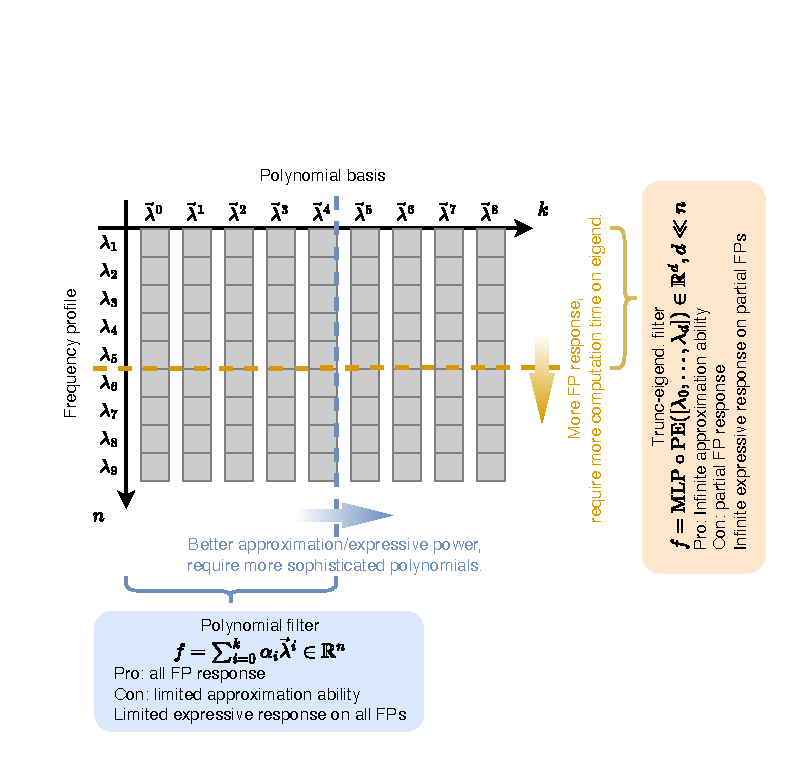
\includegraphics[width=0.7\textwidth]{figure/poly_trunc2}
	\caption{The comparison between polynomial filter and trunc-eigend. filter.}
	\label{fig:spec_expr}
\end{figure*}



\section{title}


Do we really need $U$ to be orthogonal?

As $\gL\leq\sqrt{m}\left\|\vy-\rmM\vh\right\|_2$, let $\bar\gL=\sqrt{m}\left\|\vy-\rmM\vh\right\|_2$.
\begin{proposition}
	\label{prop:relaxed_fitting}
	Given a group of $k+1$ linear independent vectors, let $U^{(k)}=\left(\vu_1,\dots,\vu_k\right)\in\sR^{n\times k}$, $U^{(k+1)}=\left(\vu_1,\dots,\vu_{k+1}\right)\in\sR^{n\times(k+1)}$ and $\rmM^{(k)}=U^{(k)}\mathrm{diag}\left(\valpha\right)U^{(k)\top}$.
	Then we have
	\begin{equation}
		\begin{aligned}
			\min_{\valpha}\bar\gL_{\rmM^{(k+1)}}\leq\min_{\valpha}\bar\gL_{\rmM^{(k)}}.
		\end{aligned}
	\end{equation}
	When $k=n$, we have $\min_{\valpha}\bar\gL_{M^{(k)}}=0$.
\end{proposition}
We prove Proposition~\ref{prop:relaxed_fitting} in Appendix~\ref{sec:relaxed_fitting}.


\section{Experiments}


\section{Conclusion}



\bibliography{reference}
\bibliographystyle{iclr2024_conference}


\appendix

\section{Proof of Proposition.~\ref{prop:loss_bound}}
\label{sec:deriviation}

%\begin{equation}
%	\begin{aligned}
%		\gL&=\left\|T\left(\vy-\rmM\vh\right)\right\|_2\\
%		&\leq\left\|T\right\|_F\left\|\vy-\rmM\vh\right\|_2\\
%		&=\sqrt{m}\left\|UU^{\top}\vy-U\mathrm{diag}\left(\vt\right)U^{\top}\vh\right\|_2\\
%		&\leq\sqrt{m}\left\|U\right\|_F\left\|U^{\top}\vy-\mathrm{diag}\left(\vt\right)U^{\top}\vh\right\|_2\\
%		&=\sqrt{m}\sqrt{n}\left\|U^{\top}\vy-\mathrm{diag}\left(U^{\top}\vh\right)\vt\right\|_2\\
%		&=\sqrt{m}\sqrt{n}\left\|\mathrm{diag}\left(U^{\top}\vh\right)\left(\mathrm{diag}^{-1}\left(U^{\top}\vh\right)U^{\top}\vy-\vt\right)\right\|_2\\
%		&\leq\sqrt{m}\sqrt{n}\left\|U^{\top}\vh\right\|_2\left\|\left(U^{\top}\vh\right)^{-1}\odot\left(U^{\top}\vy\right)-\vt\right\|_2\\
%		&\leq\sqrt{m}n\left\|\vh\right\|_2\left\|\left(U^{\top}\vh\right)^{-1}\odot\left(U^{\top}\vy\right)-\vt\right\|_2\\
%		&\leq\sqrt{m}n\eta\left\|\left(U^{\top}\vh\right)^{-1}\odot\left(U^{\top}\vy\right)-\vt\right\|_2
%	\end{aligned}
%\end{equation}


\begin{equation}
	\begin{aligned}
		\gL&=\left\|T\left(Y-\rmM H\right)\right\|_F\\
		&\leq\left\|T\right\|_F\left\|Y-\rmM H\right\|_F\\
		&=\sqrt{m}\left\|UU^{\top}Y-U\mathrm{diag}\left(\vt\right)U^{\top}H\right\|_F\\
		&\leq\sqrt{m}\left\|U\right\|_F\left\|U^{\top}Y-\mathrm{diag}\left(\vt\right)U^{\top}H\right\|_F\\
		&=\sqrt{m}\sqrt{n}\sqrt{\sum_{i=1}^c\left\|U^{\top}Y_i-\mathrm{diag}\left(\vt\right)U^{\top}H_i\right\|^2_2}\\
		&\leq\sqrt{m}\sqrt{n}\sum_{i=1}^c\left\|U^{\top}Y_i-\mathrm{diag}\left(U^{\top}H_i\right)\vt\right\|_2\\
		&=\sqrt{m}\sqrt{n}\sum_{i=1}^c\left\|\mathrm{diag}\left(U^{\top}H_i\right)\left(\mathrm{diag}^{-1}\left(U^{\top}H_i\right)U^{\top}Y_i-\vt\right)\right\|_2\\
		&\leq\sqrt{m}\sqrt{n}\sum_{i=1}^c\left\|U^{\top}H_i\right\|_2\left\|\left(U^{\top}H_i\right)^{-1}\odot\left(U^{\top}Y_i\right)-\vt\right\|_2\\
		&\leq\sqrt{m}\sqrt{n}\sum_{i=1}^c\left\|U^{\top}\right\|_F\left\|H_i\right\|_2\left\|\left(U^{\top}H_i\right)^{-1}\odot\left(U^{\top}Y_i\right)-\vt\right\|_2\\
		&=\sqrt{m}n\sum_{i=1}^c\left\|H_i\right\|_2\left\|\left(U^{\top}H_i\right)^{-1}\odot\left(U^{\top}Y_i\right)-\vt\right\|_2\\
		&\leq\sqrt{m}n\eta\sum_{i=1}^c\left\|\left(U^{\top}H_i\right)^{-1}\odot\left(U^{\top}Y_i\right)-\vt\right\|_2
	\end{aligned}
\end{equation}

\section{Proof of Proposition~\ref{prop:gc_fitting}}
\label{sec:gc_fitting}
\begin{equation}
	\begin{aligned}
		\min_{\valpha}\bar\gL_{g^{(k)}}&=\min_{\alpha_0,\dots\alpha_k}\sqrt{m}n\eta\left\|\left(U^{\top}\vh\right)^{-1}\odot\left(U^{\top}\vy\right)-g_{\valpha}^{(k)}(\vlambda)\right\|_2\\
		&=\min_{\alpha_0,\dots\alpha_k}\sqrt{m}n\eta\left\|\left(U^{\top}\vh\right)^{-1}\odot\left(U^{\top}\vy\right)-\sum_{i=0}^k\alpha_i\vlambda^i\right\|_2\\
		&=\min_{\alpha_0,\dots\alpha_k|\alpha_{k+1}=0}\sqrt{m}n\eta\left\|\left(U^{\top}\vh\right)^{-1}\odot\left(U^{\top}\vy\right)-\sum_{i=0}^{k+1}\alpha_i\vlambda^i\right\|_2\\
		&\geq\min_{\alpha_0,\dots\alpha_{k+1}}\sqrt{m}n\eta\left\|\left(U^{\top}\vh\right)^{-1}\odot\left(U^{\top}\vy\right)-\sum_{i=0}^{k+1}\alpha_i\vlambda^i\right\|_2\\
		&=\min_{\alpha_0,\dots\alpha_{k+1}}\sqrt{m}n\eta\left\|\left(U^{\top}\vh\right)^{-1}\odot\left(U^{\top}\vy\right)-g_{\valpha}^{(k+1)}(\vlambda)\right\|_2\\
		&=\min_{\valpha}\bar\gL_{g^{(k+1)}}
	\end{aligned}
\end{equation}

With $g_{\valpha}^{(n-1)}(\vlambda)=\sum_{i=0}^{n-1}\alpha_i\vlambda^i=\left(\vlambda^0,\vlambda^1,\dots\vlambda^{n-1}\right)\valpha$, consider the linear system $\left(\vlambda^0,\vlambda^1,\dots\vlambda^{n-1}\right)\valpha=\left(U^{\top}\vh\right)^{-1}\odot\left(U^{\top}\vy\right)$.
When $\vlambda$ has no repeated entries, $\left(\vlambda^0,\vlambda^1,\dots\vlambda^{n-1}\right)$ is a Vandermonde matrix with the rank equal to $n$.
Hence, a solution $\valpha_0$ always exists.
Hence
\begin{equation}
	\begin{aligned}
		\min_{\valpha}\bar\gL_{g^{(n)}}&=\min_{\alpha_0,\dots\alpha_{n-1}}\sqrt{m}n\eta\left\|\left(U^{\top}\vh\right)^{-1}\odot\left(U^{\top}\vy\right)-g_{\valpha}^{(n-1)}(\vlambda)\right\|_2\\
		&=\sqrt{m}n\eta\left\|\left(U^{\top}\vh\right)^{-1}\odot\left(U^{\top}\vy\right)-\left(\vlambda^0,\vlambda^1,\dots\vlambda^{n-1}\right)\valpha_0\right\|_2\\
		&=0.
	\end{aligned}
\end{equation}

\section{Proof of Proposition~\ref{prop:trunc_fitting}}
\label{sec:trunc_fitting}
Let $\epsilon>0$ denotes the approximation error of MLP.
Then
\begin{equation}
	\begin{aligned}
		\gL&\leq\sqrt{m}n\eta\left\|\left(U^{\top}\vh\right)^{-1}\odot\left(U^{\top}\vy\right)-\vt\right\|_2\\
		&=\sqrt{m}n\eta\left\|\left(U^{\top}\vh\right)^{-1}\odot\left(U^{\top}\vy\right)-\left(\mathrm{MLP}\left(\tilde\vlambda\right),\mathbf 0\right)\right\|_2\\
		&=\sqrt{m}n\eta\sqrt{\left\|\left(\tilde U^{\top}\vh\right)^{-1}\odot\left(\tilde U^{\top}\vy\right)-\mathrm{MLP}\left(\tilde\vlambda\right)\right\|_2^2+\left\|\left(\tilde U^{\prime\top}\vh\right)^{-1}\odot\left(\tilde U^{\prime\top}\vy\right)-\mathbf 0\right\|_2^2}\\
		&\leq\sqrt{m}n\eta\sqrt{\epsilon^2+\left\|\left(\tilde U^{\prime\top}\vh\right)^{-1}\odot\left(\tilde U^{\prime\top}\vy\right)\right\|_2^2}\\
		&\leq\sqrt{m}n\eta\left(\epsilon+\left\|\left(\tilde U^{\prime\top}\vh\right)^{-1}\odot\left(\tilde U^{\prime\top}\vy\right)\right\|_2\right).
	\end{aligned}
\end{equation}

\section{Proof of Proposition~\ref{prop:relaxed_fitting}}
\label{sec:relaxed_fitting}

\begin{equation}
	\begin{aligned}
		\min_{\valpha}\bar\gL_{\rmM^{(k+1)}}&=\min_{\valpha}\sqrt{m}\left\|\vy-\rmM^{(k+1)}\vh\right\|_2\\
		&=\min_{\alpha_0,\dots\alpha_{k+1}}\sqrt{m}\left\|\vy-\sum_{i=1}^{k+1}\valpha_iU_iU_i^{\top}\vh\right\|_2\\
		&\leq\min_{\alpha_0,\dots\alpha_k|\alpha_{k+1}=0}\sqrt{m}\left\|\vy-\sum_{i=1}^{k+1}\valpha_iU_iU_i^{\top}\vh\right\|_2\\
		&=\min_{\alpha_0,\dots\alpha_k}\sqrt{m}\left\|\vy-\sum_{i=1}^k\valpha_iU_iU_i^{\top}\vh\right\|_2\\
		&=\min_{\valpha}\sqrt{m}\left\|\vy-\rmM^{(k)}\vh\right\|_2\\
		&=\min_{\valpha}\bar\gL_{\rmM^{(k)}}
	\end{aligned}
\end{equation}
When $k=n$, $\rmM^{(n)}\vh=U\mathrm{diag}(\valpha)U^{\top}\vh=U\left(\valpha\odot U^{\top}\vh\right)$.
Let $\vx=\valpha\odot U^{\top}\vh$.
Consider the linear system $U\vx=\vy$.
As $\mathrm{rank}(U)=n$, a solution $\vx_0$ always exists.
Suppose $U_i^{\top}\vh\neq0$ for all $i\in[n]$.
Correspondingly, $\valpha_0=\vx_0\odot\left(U^{\top}\vh\right)^{-1}$.
Therefore, $\min_{\valpha}\bar\gL_{\rmM^{(n)}}=\bar\gL_{\rmM^{(n)}}\big|_{\valpha_0}=0$.


\newpage

\section{MISC}

$H$ is channel-independent.
$\vt$ is shared over different channels.
There are also channel-independent filter design where each signal channel learns an individual filter~\citep{yang2022spectrum,JacobiConv,bo2022specformer}.
Correspondingly, the loss is $\gL\leq\sqrt{m}n\eta\sum_{i=1}^c\left\|\left(U^{\top}H_i\right)^{-1}\odot\left(U^{\top}Y_i\right)-\rmT_i\right\|_F$ with $\rmT\in\sR^{n\times c}$.

\subsection{Exploring graph representation space}
According to spectral theorem $\rmM=U\mathrm{diag}(\vt)U^{\top}$, a graph matrix representation $\rmM$ provides a unique tuple $(U,\vt)$.
$(U,\vt)$ decides the fitting ability.
Improving fitting ability while maintaining graph topology information.

\begin{equation}
	\begin{aligned}
		\gL&=\left\|T\left(Y-\rmM H\right)\right\|_F\\
		&\leq\left\|T\right\|_F\left\|Y-\rmM H\right\|_F\\
		&=\left\|T\right\|_F\left\|Y-\sum_{i=1}^n\vlambda_iU_iU_i^{\top}H\right\|_F\\
		&=\left\|T\right\|_F\left\|\sum_{i=1}^nU_iU_i^{\top}Y-\sum_{i=1}^n\vlambda_iU_iU_i^{\top}H\right\|_F\\
		&=\left\|T\right\|_F\left\|\sum_{i=1}^nU_iU_i^{\top}\left(Y-\vlambda_iH\right)\right\|_F\\
		&\leq\left\|T\right\|_F\sum_{i=1}^n\left\|U_iU_i^{\top}\left(Y-\vlambda_iH\right)\right\|_F\\
		&=\left\|T\right\|_F\sum_{i=1}^n\sqrt{\sum_{j=1}^c\left\|U_iU_i^{\top}\left(Y_j-\vlambda_iH_j\right)\right\|^2_F}\\
		&=\left\|T\right\|_F\sum_{i=1}^n\sqrt{\sum_{j=1}^c\left(U_i^{\top}\left(Y_j-\vlambda_iH_j\right)\right)^2\left\|U_i\right\|^2_F}\\
		&=\left\|T\right\|_F\sum_{i=1}^n\sqrt{\sum_{j=1}^c\left(U_i^{\top}\left(Y_j-\vlambda_iH_j\right)\right)^2}
	\end{aligned}
\end{equation}

\begin{equation}
	\begin{aligned}
		\gL&=\left\|T\left(Y-\rmM H\right)\right\|_F\\
		&\leq\left\|T\right\|_F\left\|Y-\rmM H\right\|_F\\
		&=\sqrt{m}\left\|UU^{\top}Y-U\mathrm{diag}\left(\vt\right)U^{\top}H\right\|_F\\
		&\leq\sqrt{m}\left\|U\right\|_F\left\|U^{\top}Y-\mathrm{diag}\left(\vt\right)U^{\top}H\right\|_F\\
		&=\sqrt{m}\sqrt{n}\sqrt{\sum_{j=1}^c\left\|U^{\top}Y_j-\mathrm{diag}\left(\vt\right)U^{\top}H_j\right\|^2_F}\\
		&=\sqrt{m}\sqrt{n}\sqrt{\sum_{j=1}^c\left\|U^{\top}Y_j-\mathrm{diag}\left(U^{\top}H_j\right)\vlambda\right\|^2_F}\\
		&=\sqrt{m}\sqrt{n}\sqrt{\sum_{j=1}^c\left\|\mathrm{diag}\left(U^{\top}H_j\right)\left(\mathrm{diag}^{-1}\left(U^{\top}H_j\right)U^{\top}Y_j-\vlambda\right)\right\|^2_F}\\
		&\leq\sqrt{m}\sqrt{n}\sqrt{\sum_{j=1}^c\left\|U^{\top}H_j\right\|^2_F\left\|\left(U^{\top}H_j\right)^{-1}\odot\left(U^{\top}Y_j\right)-\vlambda\right\|^2_F}\\
		&\leq\sqrt{m}\sqrt{n}\sqrt{\sum_{j=1}^c\left\|U^{\top}\right\|^2_F\left\|H_j\right\|^2_F\left\|\left(U^{\top}H_j\right)^{-1}\odot\left(U^{\top}Y_j\right)-\vlambda\right\|^2_F}\\
		&=\sqrt{m}n\sqrt{\sum_{j=1}^c\left\|H_j\right\|^2_F\left\|\left(U^{\top}H_j\right)^{-1}\odot\left(U^{\top}Y_j\right)-\vlambda\right\|^2_F}\\
		&\leq\sqrt{m}n\sum_{j=1}^c\left\|H_j\right\|_F\left\|\left(U^{\top}H_j\right)^{-1}\odot\left(U^{\top}Y_j\right)-\vlambda\right\|_F
	\end{aligned}
\end{equation}

\end{document}
